\section{香港真的有高度自治嗎?}
\label{sec:sec16}

表面上,香港擁有極高的自治權,甚至比世界上許多自治政體還要高。實際上,香港的自治權恐怕比美國聯邦制下的一個州還要低。這個落差,源自於香港高度自治的本質和目的。

從政治學去看,討論自治政體的權力離不開以下五點:自治政體的地位和權力的來源;自治政體本身的政府如何組成;自治政體如何參與全國事務;當自治政體與中央政府出現矛盾時由誰來訟裁;以及自治政體與中央政府如何分權。香港的問題,在於除了在分權這一項優於世界上其他自治政體之外,各方面都要來的糟糕。

先談自治政體的設立。以美國的聯邦制為例,州政府和聯邦政府的權責按美國《憲法》第十修正案規定:「憲法未授予合眾國、也未禁止各州行使的權力,由各州各自保留,或由人民保留」。在此制度下,各州政府的權力受到相對明確的保障。如要根本改變州政府和聯邦政府的關係,則要修改《憲法》才可發生。相反,在一個單一制的國家,例如英國,國會就有遠遠較多的權力去改變中央與地方的關係。例如英國曾經在一九八六年直接廢除了大倫敦議會(Greater London Council),使得倫敦市陷入「無政府狀態」,只靠倫敦範圍內各行政區互相協調來管理。到了二零零零年,英國又重新設立大倫敦政府(Greater London Authority),並設直選倫敦市長一職。這些改變都只要國會通過就可以實行。當然,英國政府願意恢復倫敦的地位,是因為國會競選時英國工黨承諾如果當選則會推行此政策,於是在選舉中獲得倫敦市民支持。

相比較之下,香港特別行政區是由全國人民代表大會按中國《憲法》第三十一條設立,而憲法條文本身並無明確規定特別行政區的權力範圍。中國作為一個單一制國家,而全國人民代表大會的決定普遍都以九成以上的票數通過,香港特別行政區在中國國內的法理保障其實十分有限。

說到自治政體本身的政府如何組成,香港的自治程度不單比美國聯邦制下的地方政府低,也比單一制下英國的大倫敦政府還要差。香港的行政長官要履行權力時,面對的限制十分之多,其中以雙重效忠的問題最為明顯。《基本法》第四十三條規定:「香港特別行政區行政長官依照本法的規定對中央人民政府和香港特別行政區負責」。這條條文看起來沒有什麼特別,但相對於其他國家的中央與地方關係,則十分奇怪。

以紐約市政府的組織架構圖為例,放在最高位置的並非市長,而是「紐約市全體人民」。換言之,紐約市市長要向紐約市市民負責。在這組織架構圖當中,紐約州州長或美國總統都沒有位置。這不是說他們不能影響到紐約市政府的運作,而是說他們和紐約市政府之間沒有從屬關係。紐約市市長可以也經常公開批評美國總統,當美國總統的決定不符合紐約市市民的利益時會清楚表明,從來不會有人覺得他這樣做會威脅得到美國總統的威嚴,更不會有人將之引伸為紐約市要搞分裂。反過來說,美國總統如對紐約市市長有任何不滿,也不能直接把紐約市長革走,因為紐約市政府的權力架構本身和聯邦政府無關。

\begin{figure}[htbp]
    \centering
    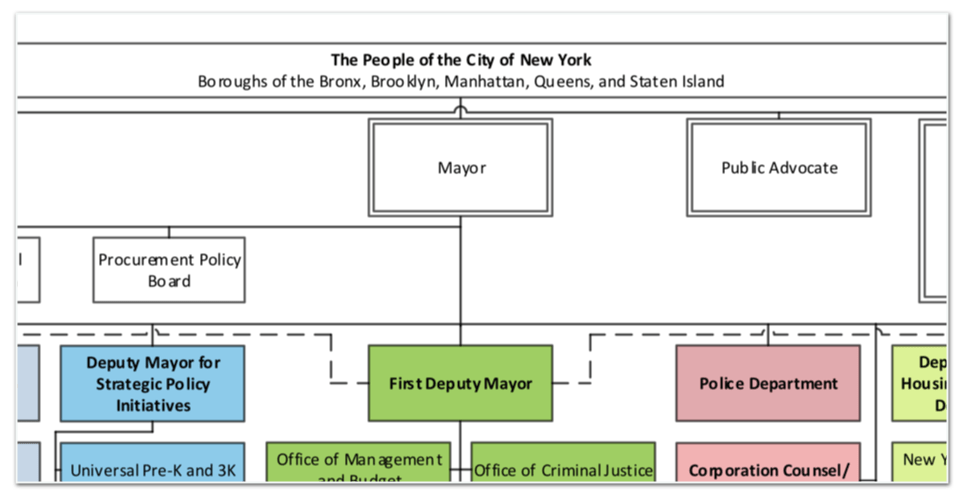
\includegraphics[width=0.7\textwidth]{c16/h-klesson1-023.png}
    \caption{紐約市組織圖(部份)} 
\end{figure}

即使在單一制的英國,倫敦市長即不由國會直接問責,也不用向英國首相述職。他要和西敏寺建立一個怎樣的關係才能最大程度保障倫敦市民的利益,是他的選擇。當然,理論上如果英國國會不高興,可以把整個倫敦市長的職位廢除。不過一旦制度設立了,就得按制度行事,不存在日常意義下的從屬關係。

但在香港,中央政府對香港政府的影響力就遠遠大得多。《基本法》列明行政長官既要向中央政府負責,又要向香港特區負責。如是者,當中央政府和香港特區的利益出現矛盾時,行政長官該怎麼辦就成為難題。中央政府和香港特區有利益矛盾,不一定是中央政府刻意要難為香港特區,也不一定是香港特區刻意要挑戰中央政府。就算中央政府的出發點是為香港特區的利益著想,香港社會的想法也未必一樣,一個人眼中的禮物在另一個人的眼中可變成廢物,本來是一件很正常的事情。

經過二十年的實際操作,上述矛盾的後果十分明顯:行政長官會完全倒向中央政府的一邊。無論是《基本法》的規定或是非正規的政治操作中,中央政府都有很多渠道向行政長官施壓;相反,香港社會即使對行政長官有多大的不滿,也不太可能直接挑戰。按《基本法》第五十條和第七十九條第九項的規定,行政長官選出後要得到中央政府的任命,而即使被立法會彈劾也要待中央政府決定去留。也就是說,中央政府有權否決香港選舉出來的行政長官人選,也有權否決立法會對行政長官的彈劾。如是者,「對中央人民政府和香港特別行政區負責」這句話的下半其實是虛文,只有上半是真的。

相對來說,美國國會固然沒有任命紐約市長的權力,英國國會也不能否決倫敦市長選舉的當選人成為倫敦市長。這點十分重要,因為它確保了權力分立和互相制衡:當美國總統特朗普因為他過去和俄羅斯的官商關係而被聯邦特別檢察官調查時,理論上他可以總統身分要求他的下屬把檢察官革職。不過,這樣做不能完全終止調查,因為涉及的罪行如洗黑錢等在州政府的層面同樣違法,可由州政府接手調查,特朗普對此就無能為力。這個制度區隔為總統濫權提供了重要制衡。換轉在香港,如果香港政府要調查中央政府要員在香港有否從事非法經濟活動,實際上就極為困難,而這正正顯示出兩者自治程度的區別。

至於自治政體如何參與全國事務以及當自治政體與中央政府出現矛盾時由誰來訟裁,香港的情況相對於其他自治政體來說也不理想。紐約市民如果不滿美國聯邦政府,可以在國會和總統選舉中投票;倫敦市民如果不滿英國政府,也可以在國會選舉中投票。然而全國人民代表大會當中的香港代表並非由香港人普遍選舉產生,而是由過去各屆的選舉委員會成員投票產生。選舉委員會在香港社會的代表性本來就極受爭議,所以港區人大代表在香港的代表性同樣不被普遍認同(見\hyperref[sec:sec18]{問題十八})。民間交流方面,中國政府又大力阻擋香港人通過非政府組織介入中國大陸事務,擔心香港成為「反共基地」。如是者,中港之間就出現了全國政治可以干預地方政治,地方政治卻不可以參與全國政治的一面倒關係。

至於爭議訟裁方面,《基本法》本來對此特別是對釋法權有一系列的說明(見\hyperref[sec:sec25]{問題二十五}),但實行起來卻變成人大常委可作不受制約的決定。相對來說,美國各州如認為聯合政府的決定越權,侵犯到該州利益,大可以到聯邦法院起訴,通過獨立的司法程序來處理。在中國,最高人民法院本身從屬於全國人大,也沒有中國公民在最高人民法院成功起訴國務院的案例。在爭議訟裁這方面,香港的高度自治同樣比美國的聯邦制更欠保障。

香港在制度上唯一比其他自治政體優勝之處,在於如何與中央政府分權,雖然在這方面也存在明顯理想與現實間的落差。按照《基本法》,除了外交和國防以外,特區政府可以全面管理各種內部事務,可以發行自己的護照和貨幣,又不用向中央政府交稅,更可參加各個國際組織和與外國商討貿易協定。表面上,香港特區的權力遠高於世界上其他的自治政體。

不過,現實中的香港政府未必能實踐這些條文上的自主。首先,由於行政長官本身由中央政府任命,難以想像行政長官在處理各種涉外政策時會違反中央政府的意願(相反,加州州長卻會繞過美國總統自己走去外國討論氣候變遷)。不僅是行政長官,主要官員也要得到中央政府的任命,即中央政府有權否決主要官員的人選。如果中央政府把這規定所包含的權力用盡的話,可以輕易介入香港特區各項原屬自治範圍的事務,如可以通過對教育局長的任免權力直接影響到香港的教育政策,儘管教育政策與外交和國防事務無關。這樣去看,條文上香港特區所得的分權雖然很多,但實行起來的自主性卻比其他自治政體還要低。最起碼,紐約州教育委員會的成員是由紐約州議會選出,並非由聯邦政府任命,自然就不用好像香港政府那樣一收到中央政府的要求後便要大搞國民教育。

\begin{figure}[htbp]
    \centering
    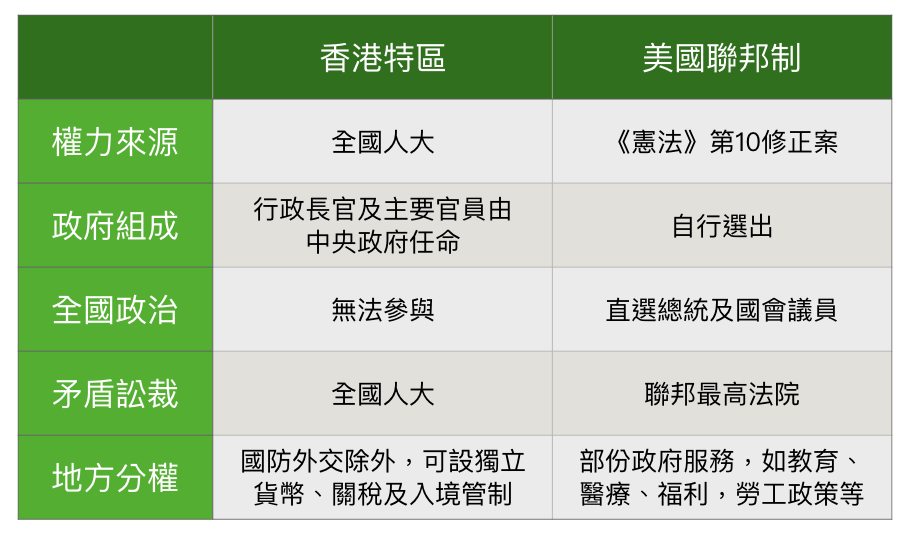
\includegraphics[width=0.7\textwidth]{c16/h-klesson1-022.png}
    \caption{比較香港的「一國兩制」和美國的聯邦制} 
\end{figure}

順帶一提,《基本法》不少條文對於中港之間的分權其實寫得不太清楚,特別是在涉外關係的部分。例如《基本法》第一百五十四條列明「香港特別行政區政府可實行出入境管制」,當中「可」這個字就很值得細心思考。條文說香港政府可以實行出入境管制,但沒有說只有香港政府才可以,也沒有說中央政府不可以。於是乎,條文可被理解為這個權力不是絕對的,中央政府有干預香港出入境管制的平行權力(雖然按中國政府自己的慣例,一個機構授權予另一機構後,自己就不會再同時執行這個權力)。現實上,中國政府已有多次以政治理由干預香港是否容許外國人入境的紀錄,對象包括外國議員和異見人士。

當然,對於一個地方政府來說,可合理認為它和中央政府的關係不應時時弄得太僵,就算沒有明文規定也應避免無謂衝突。但這是出於地方政府的自我選擇,還是出於中央政府的強制要求,對建立管治認授有莫大分別。把地方首長服從中央政府寫成法律條文,而地方民眾又無權參與中央政府的組成時,地方政府認授低落就是一個很合理的後果,各種管治困難也會隨之而來。

香港特區政府並非由香港人普遍選出;香港人普遍不能參與全國事務;《基本法》是中國《憲法》下的專法,地位低於《憲法》;如有爭議,則由人大常委這個政治機構說了算,而不是獨立的法院。在這一系列的制度安排之下,香港特區的高度自治更大程度上是中央政府製造出來方便中國和國際社會交往的白手套,多於實際保證港人治港不受干擾的相互協訂。

\rule[-10pt]{15cm}{0.05em}

伸延閱讀:

Gittings D (2016) A High Degree of Autonomy?, \textit{Introduction to the Hong Kong Basic Law (2nd Edition)}. Hong Kong University Press.

Chen AHY (2018) The autonomy of Hong Kong under “One Country, Two Systems”, \textit{Routledge Handbook of Contemporary Hong Kong}. New York: Routledge.